%%%%%%%%%%%%%%%%%%%%%%%%%%%%%%%%%%%%%%%%%%%%%%%%%%%%%%%%%%%%%%%%%%%%%%%%%%%%%%%%%%%%%%%%%%%%%%%%%%%%%%%%%%%%%%%%%%%%%%%%%%%%%%%%%%%%%%%%%%%%%%%%%%%%%%%%%%%
% This is just an example/guide for you to refer to when producing your supplementary material for your Frontiers article.                                 %
%%%%%%%%%%%%%%%%%%%%%%%%%%%%%%%%%%%%%%%%%%%%%%%%%%%%%%%%%%%%%%%%%%%%%%%%%%%%%%%%%%%%%%%%%%%%%%%%%%%%%%%%%%%%%%%%%%%%%%%%%%%%%%%%%%%%%%%%%%%%%%%%%%%%%%%%%%%

%%% Version 2.4 Generated 2017/05/01 %%%
%%% You will need to have the following packages installed: datetime, fmtcount, etoolbox, fcprefix, which are normally inlcuded in WinEdt. %%%
%%% In http://www.ctan.org/ you can find the packages and how to install them, if necessary. %%%
%%%  NB logo1.jpg is required in the path in order to correctly compile front page header %%%

\documentclass[utf8]{frontiers_suppmat} % for all articles
\usepackage{url,hyperref,lineno,microtype,subcaption}
\usepackage[onehalfspacing]{setspace}
\usepackage{lscape}
\usepackage{booktabs}

\def\firstAuthorLast{Villaseñor-Derbez {et~al.}}

% Leave a blank line between paragraphs instead of using \\

\begin{document}
\onecolumn
\firstpage{1}

\title[Supplementary Material]{{\helveticaitalic{Supplementary Material}}:
\\ \helvetica{Effectiveness of community-based TURF-reserves in small-scale fisheries}} %Please insert the title of your article here


\maketitle

%%% There is no need for adding the file termination, as long as you indicate where the file is saved. In the examples below the files (logo1.jpg and logos.jpg) are in the Frontiers LaTeX folder
%%% If using *.tif files convert them to .jpg or .png
%%%  NB logo1.jpg is required in the path in order to correctly compile front page header %%%

Raw data and code are available on GitHub at:
\url{https://github.com/jcvdav/ReserveEffect}

\begin{table}

\caption{\label{tab:unnamed-chunk-2}Number of invertebrate transects performed in each site of each community.}
\centering
\begin{tabular}[t]{lrr}
\toprule
Community & Control & Reserve\\
\midrule
Isla Natividad & 415 & 244\\
Maria Elena & 27 & 21\\
Punta Herrero & 51 & 73\\
\bottomrule
\end{tabular}
\end{table}

\begin{figure}
\centering
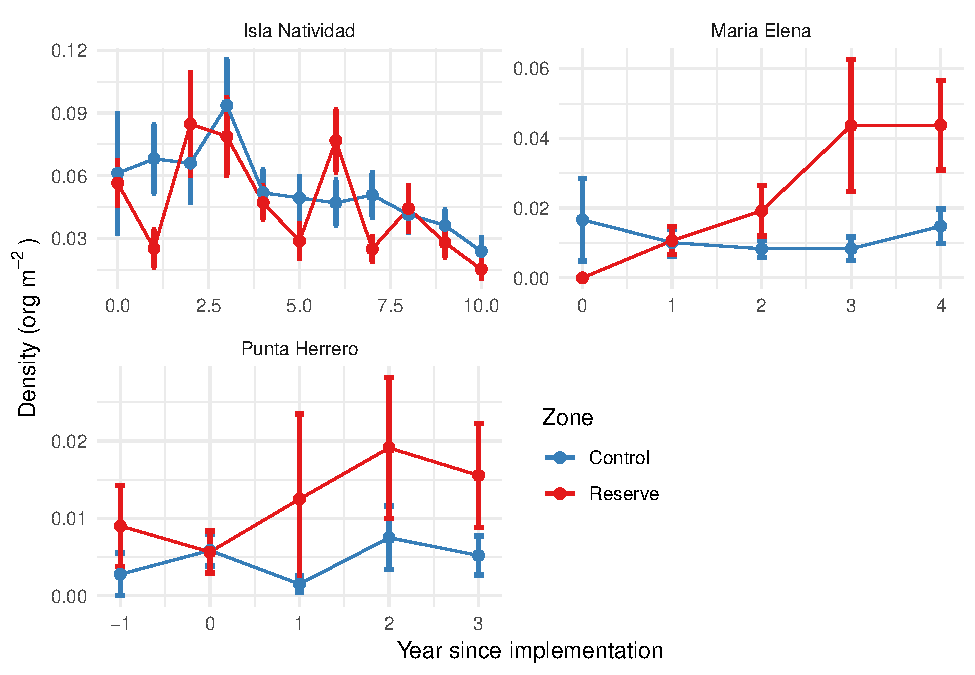
\includegraphics{SupplementaryMaterial_files/figure-latex/unnamed-chunk-3-1.pdf}
\caption{\label{fig:unnamed-chunk-3}Time series of lobster densities. Bars
indicate standard errors.}
\end{figure}

\begin{figure}
\centering
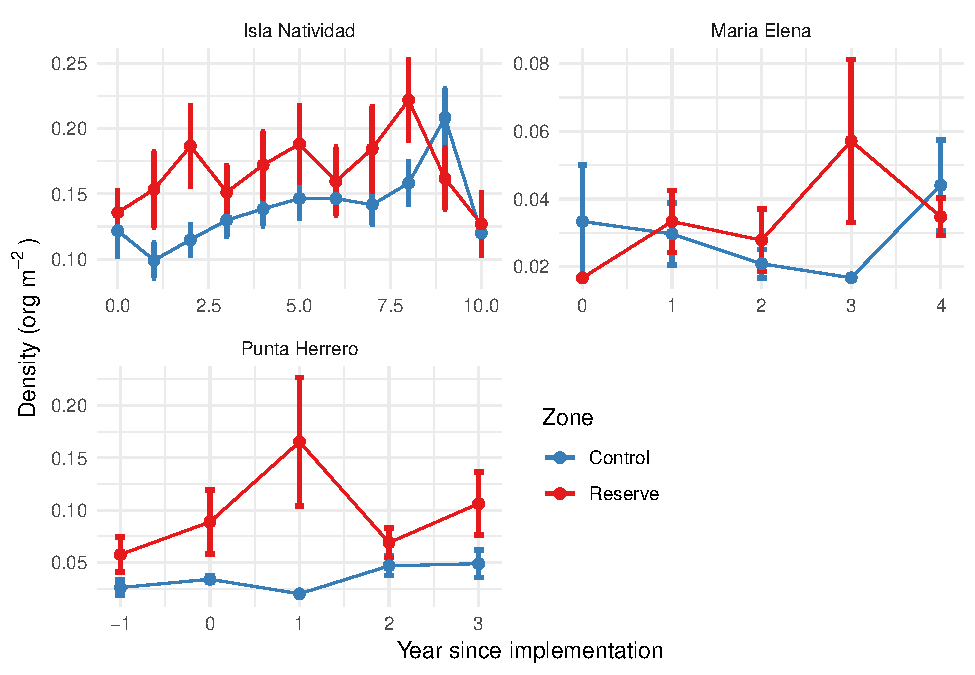
\includegraphics{SupplementaryMaterial_files/figure-latex/unnamed-chunk-4-1.pdf}
\caption{\label{fig:unnamed-chunk-4}Time series of invertebrate densities.
Bars indicate standard errors.}
\end{figure}

\clearpage

\begin{table}

\caption{\label{tab:unnamed-chunk-5}Number of fish transects performed in each site of each community.}
\centering
\begin{tabular}[t]{lrr}
\toprule
Community & Control & Reserve\\
\midrule
Isla Natividad & 400 & 241\\
Maria Elena & 44 & 45\\
Punta Herrero & 82 & 85\\
\bottomrule
\end{tabular}
\end{table}

\begin{figure}
\centering
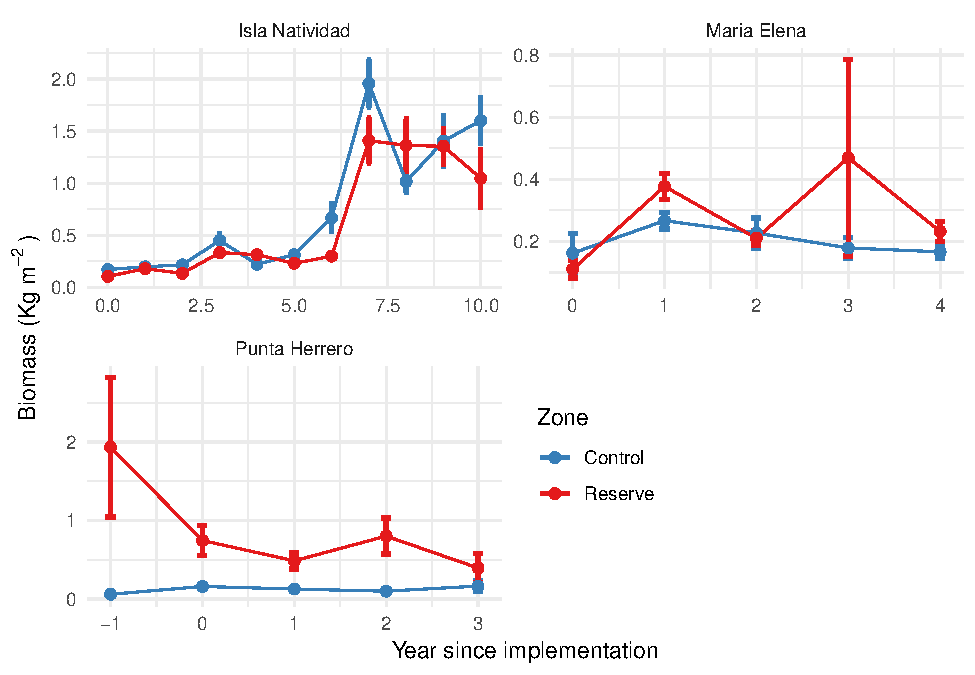
\includegraphics{SupplementaryMaterial_files/figure-latex/unnamed-chunk-6-1.pdf}
\caption{\label{fig:unnamed-chunk-6}Time series of fish biomass. Bars
indicate standard errors.}
\end{figure}

\clearpage

\begin{figure}
\centering
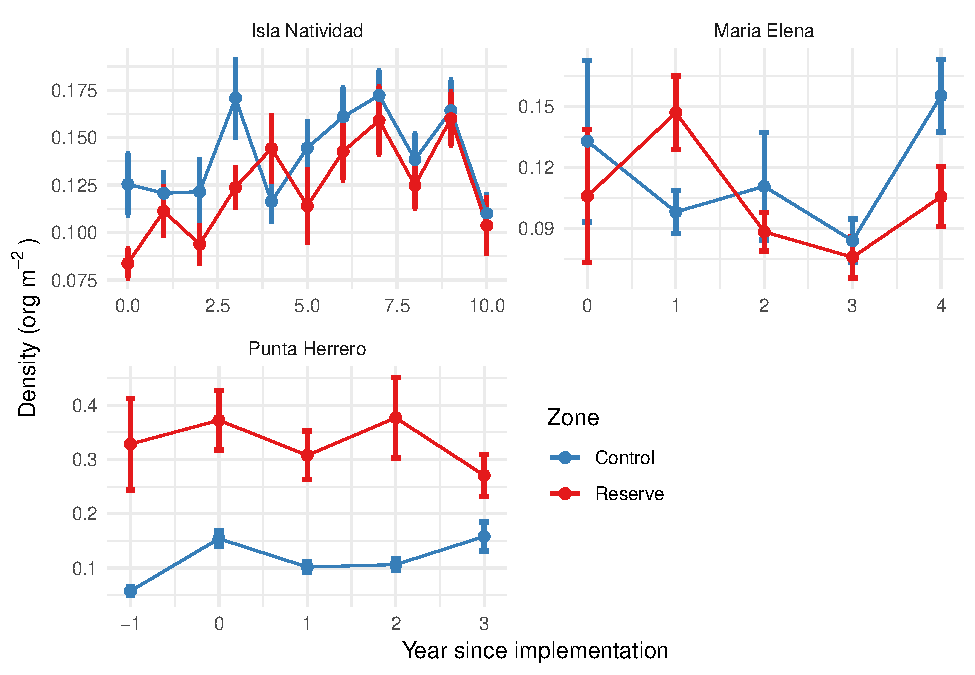
\includegraphics{SupplementaryMaterial_files/figure-latex/unnamed-chunk-7-1.pdf}
\caption{\label{fig:unnamed-chunk-7}Time series of fish densities. Bars
indicate standard errors.}
\end{figure}

\clearpage

\begin{table}

\caption{\label{tab:unnamed-chunk-8}Mean ex-vessel prices for lobster (Panulirus spp.) on each TURF (community) by zone (MC = Caribbean; PN = Pacific) and group (Control = only TURF, Treated = TURF and reserve).}
\centering
\begin{tabular}[t]{lllrr}
\toprule
Zone & Group & TURF & Before & After\\
\midrule
MC & Control & langosteros del caribe & 165.58 & 176.72\\
MC & Control & vigia chico & 177.66 & 175.31\\
MC & Treated & cozumel & 178.21 & 170.49\\
MC & Treated & jose maria azcorra & 185.95 & 207.83\\
PN & Control & bahia tortugas & 155.60 & 122.46\\
\addlinespace
PN & Control & la purisima & 67.54 & 157.88\\
PN & Control & pesc nacionales de abulon & 67.16 & 88.79\\
PN & Treated & buzos y pescadores de la baja california & 89.35 & 190.07\\
\bottomrule
\end{tabular}
\end{table}

\begin{figure}
\centering
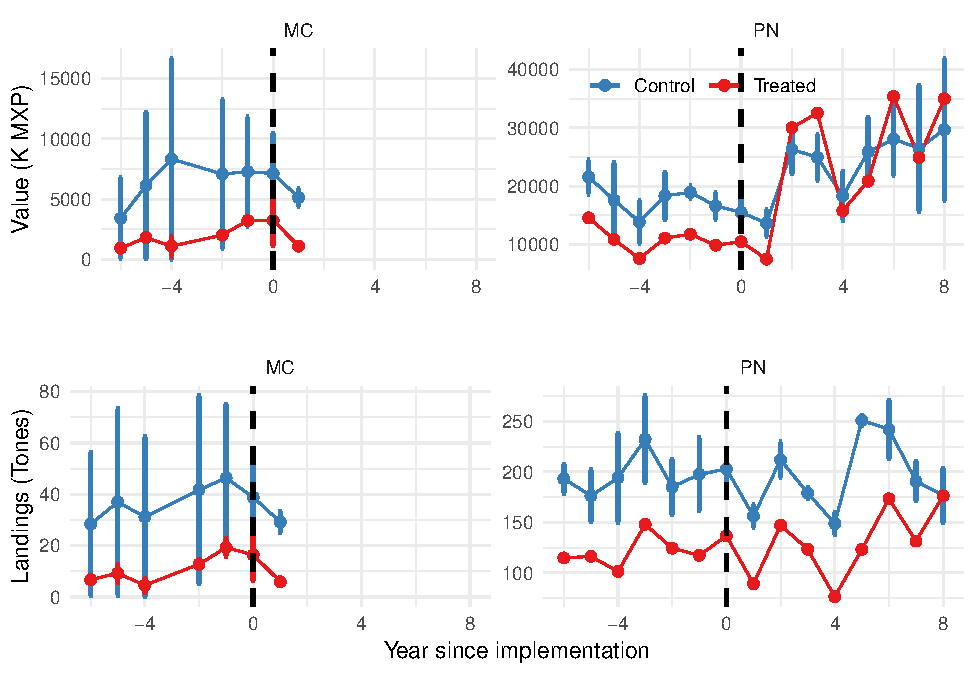
\includegraphics{SupplementaryMaterial_files/figure-latex/unnamed-chunk-9-1.pdf}
\caption{\label{fig:unnamed-chunk-9}Time series of landings and value of
landings.}
\end{figure}

\clearpage

\begin{table}[!htbp] \centering 
  \caption{Coefficient estimates of biological indicators for Isla Natividad.} 
  \label{} 
\tiny 
\begin{tabular}{@{\extracolsep{1pt}}lcccc} 
\\[-1.8ex]\hline 
\hline \\[-1.8ex] 
 & \multicolumn{4}{c}{\textit{Dependent variable:}} \\ 
\cline{2-5} 
\\[-1.8ex] & \multicolumn{4}{c}{} \\ 
 & Lobster abundance & Fish biomass & Invertebrate abundance & Invertebrate biomass \\ 
\\[-1.8ex] & (1) & (2) & (3) & (4)\\ 
\hline \\[-1.8ex] 
 zonaReserva & $-$0.011 (0.058) & $-$0.003 (0.002) & 0.002 (0.020) & $-$0.031$^{*}$ (0.017) \\ 
  year1 & 0.032 (0.067) & $-$0.004 (0.003) & $-$0.027 (0.021) & 0.001 (0.018) \\ 
  year2 & 0.0002 (0.077) & $-$0.004 (0.003) & 0.002 (0.020) & 0.010 (0.022) \\ 
  year3 & 0.023 (0.072) & 0.004 (0.003) & 0.014 (0.020) & 0.053$^{**}$ (0.025) \\ 
  year4 & $-$0.030 (0.058) & $-$0.002 (0.002) & $-$0.009 (0.020) & $-$0.005 (0.018) \\ 
  year5 & $-$0.006 (0.061) & 0.001 (0.002) & 0.006 (0.020) & 0.036$^{*}$ (0.020) \\ 
  year6 & $-$0.014 (0.062) & 0.008$^{**}$ (0.003) & 0.014 (0.020) & 0.049$^{**}$ (0.022) \\ 
  year7 & $-$0.021 (0.060) & 0.064$^{***}$ (0.010) & $-$0.044$^{*}$ (0.023) & 0.063$^{***}$ (0.019) \\ 
  year8 & $-$0.026 (0.059) & 0.027$^{***}$ (0.005) & $-$0.029 (0.020) & 0.025 (0.020) \\ 
  year9 & $-$0.038 (0.057) & 0.040$^{***}$ (0.009) & $-$0.021 (0.025) & 0.056$^{**}$ (0.022) \\ 
  year10 & $-$0.066 (0.057) & 0.043$^{***}$ (0.009) & $-$0.107$^{***}$ (0.024) & $-$0.006 (0.018) \\ 
  zonaReserva:year1 & $-$0.058 (0.078) & 0.005 (0.004) & 0.041 (0.031) & 0.013 (0.023) \\ 
  zonaReserva:year2 & 0.126 (0.121) & 0.005 (0.004) & 0.049 (0.033) & 0.007 (0.024) \\ 
  zonaReserva:year3 & 0.053 (0.093) & 0.001 (0.004) & 0.004 (0.027) & $-$0.020 (0.028) \\ 
  zonaReserva:year4 & 0.035 (0.065) & 0.007$^{**}$ (0.003) & 0.017 (0.030) & 0.075$^{***}$ (0.025) \\ 
  zonaReserva:year5 & $-$0.045 (0.068) & 0.001 (0.004) & 0.013 (0.029) & $-$0.0003 (0.028) \\ 
  zonaReserva:year6 & 0.096 (0.075) & $-$0.001 (0.004) & 0.013 (0.029) & 0.009 (0.027) \\ 
  zonaReserva:year7 & $-$0.030 (0.065) & $-$0.013 (0.017) & 0.012 (0.033) & 0.008 (0.026) \\ 
  zonaReserva:year8 & 0.012 (0.069) & 0.026 (0.016) & 0.032 (0.028) & 0.021 (0.025) \\ 
  zonaReserva:year9 & 0.002 (0.064) & 0.007 (0.012) & $-$0.077$^{**}$ (0.036) & 0.031 (0.027) \\ 
  zonaReserva:year10 & $-$0.016 (0.062) & $-$0.011 (0.016) & $-$0.018 (0.034) & 0.027 (0.024) \\ 
  Constant & 0.122$^{**}$ (0.054) & 0.001 (0.006) & 0.059$^{***}$ (0.018) & 0.119$^{***}$ (0.042) \\ 
 \hline \\[-1.8ex] 
Observations & 659 & 2,987 & 3,714 & 2,987 \\ 
R$^{2}$ & 0.049 & 0.211 & 0.426 & 0.153 \\ 
Residual Std. Error & 0.189 (df = 637) & 0.067 (df = 2947) & 0.187 (df = 3667) & 0.165 (df = 2947) \\ 
\hline 
\hline \\[-1.8ex] 
\textit{Note:}  & \multicolumn{4}{r}{$^{*}$p$<$0.1; $^{**}$p$<$0.05; $^{***}$p$<$0.01} \\ 
\end{tabular} 
\end{table}

\clearpage

\begin{table}[!htbp] \centering 
  \caption{Coefficient estimates of biological indicators for Maria Elena.} 
  \label{} 
\tiny 
\begin{tabular}{@{\extracolsep{1pt}}lcccc} 
\\[-1.8ex]\hline 
\hline \\[-1.8ex] 
 & \multicolumn{4}{c}{\textit{Dependent variable:}} \\ 
\cline{2-5} 
\\[-1.8ex] & \multicolumn{4}{c}{} \\ 
 & Lobster abundance & Fish biomass & Invertebrate abundance & Invertebrate biomass \\ 
\\[-1.8ex] & (1) & (2) & (3) & (4)\\ 
\hline \\[-1.8ex] 
 zonaReserva & $-$0.033$^{**}$ (0.013) & $-$0.001 (0.002) & $-$0.007 (0.021) & $-$0.024 (0.047) \\ 
  year1 & 0.008 (0.023) & 0.003$^{*}$ (0.002) & 0.010 (0.019) & $-$0.034 (0.038) \\ 
  year2 & $-$0.019 (0.015) & 0.001 (0.002) & $-$0.004 (0.015) & $-$0.037 (0.044) \\ 
  year3 & $-$0.028$^{**}$ (0.014) & $-$0.0001 (0.002) & $-$0.002 (0.016) & $-$0.057 (0.040) \\ 
  year4 & 0.023 (0.028) & 0.0004 (0.002) & 0.022 (0.022) & 0.044 (0.041) \\ 
  zonaReserva:year1 & $-$0.003 (0.024) & 0.004$^{*}$ (0.002) & 0.008 (0.023) & 0.065 (0.051) \\ 
  zonaReserva:year2 & 0.046$^{*}$ (0.024) & 0.002 (0.002) & 0.017 (0.022) & 0.020 (0.053) \\ 
  zonaReserva:year3 & 0.074$^{***}$ (0.024) & 0.001 (0.002) & 0.039 (0.040) & 0.013 (0.049) \\ 
  zonaReserva:year4 & 0.001 (0.031) & 0.003 (0.002) & $-$0.001 (0.027) & $-$0.040 (0.052) \\ 
  Constant & 0.033$^{**}$ (0.013) & $-$0.0004 (0.001) & 0.010 (0.019) & 0.133$^{***}$ (0.040) \\ 
 \hline \\[-1.8ex] 
Observations & 48 & 1,146 & 75 & 1,146 \\ 
R$^{2}$ & 0.222 & 0.807 & 0.199 & 0.248 \\ 
Residual Std. Error & 0.038 (df = 38) & 0.010 (df = 1090) & 0.035 (df = 57) & 0.175 (df = 1090) \\ 
\hline 
\hline \\[-1.8ex] 
\textit{Note:}  & \multicolumn{4}{r}{$^{*}$p$<$0.1; $^{**}$p$<$0.05; $^{***}$p$<$0.01} \\ 
\end{tabular} 
\end{table}

\clearpage

\begin{table}[!htbp] \centering 
  \caption{Coefficient estimates of biological indicators for Punta Herrero.} 
  \label{} 
\small 
\begin{tabular}{@{\extracolsep{1pt}}lcccc} 
\\[-1.8ex]\hline 
\hline \\[-1.8ex] 
 & \multicolumn{4}{c}{\textit{Dependent variable:}} \\ 
\cline{2-5} 
\\[-1.8ex] & \multicolumn{4}{c}{} \\ 
 & Lobster abundance & Fish biomass & Invertebrate abundance & Invertebrate biomass \\ 
\\[-1.8ex] & (1) & (2) & (3) & (4)\\ 
\hline \\[-1.8ex] 
 zonaReserva & 0.004 (0.009) & 0.014$^{**}$ (0.005) & 0.069$^{**}$ (0.035) & 0.170$^{***}$ (0.054) \\ 
  year-1 & $-$0.006 (0.007) & $-$0.001 (0.002) & 0.019 (0.022) & $-$0.087$^{***}$ (0.031) \\ 
  year1 & $-$0.008 (0.005) & $-$0.003 (0.002) & $-$0.0001 (0.018) & $-$0.073$^{***}$ (0.028) \\ 
  year2 & 0.004 (0.009) & $-$0.002 (0.002) & 0.032$^{**}$ (0.014) & $-$0.053$^{*}$ (0.028) \\ 
  year3 & $-$0.001 (0.006) & $-$0.002 (0.002) & 0.038$^{*}$ (0.020) & $-$0.016 (0.032) \\ 
  zonaReserva:year-1 & 0.017 (0.023) & $-$0.013$^{*}$ (0.008) & $-$0.044 (0.043) & $-$0.134$^{*}$ (0.081) \\ 
  zonaReserva:year1 & 0.018 (0.024) & $-$0.011$^{*}$ (0.006) & 0.048 (0.071) & $-$0.021 (0.066) \\ 
  zonaReserva:year2 & 0.019 (0.021) & $-$0.001 (0.008) & $-$0.076 (0.048) & 0.032 (0.086) \\ 
  zonaReserva:year3 & 0.016 (0.016) & $-$0.013$^{*}$ (0.007) & $-$0.012 (0.047) & $-$0.110 (0.069) \\ 
  Constant & 0.011$^{**}$ (0.005) & $-$0.001 (0.002) & 0.092$^{***}$ (0.023) & 0.122$^{***}$ (0.046) \\ 
 \hline \\[-1.8ex] 
Observations & 124 & 1,628 & 262 & 1,628 \\ 
R$^{2}$ & 0.051 & 0.345 & 0.127 & 0.271 \\ 
Residual Std. Error & 0.049 (df = 114) & 0.051 (df = 1566) & 0.165 (df = 243) & 0.506 (df = 1566) \\ 
\hline 
\hline \\[-1.8ex] 
\textit{Note:}  & \multicolumn{4}{r}{$^{*}$p$<$0.1; $^{**}$p$<$0.05; $^{***}$p$<$0.01} \\ 
\end{tabular} 
\end{table}

\clearpage

\begin{table}[!htbp] \centering 
  \caption{Coefficient estimates of socioeconomic indicators Isla Natividad.} 
  \label{} 
\tiny 
\begin{tabular}{@{\extracolsep{1pt}}lcc} 
\\[-1.8ex]\hline 
\hline \\[-1.8ex] 
 & \multicolumn{2}{c}{\textit{Dependent variable:}} \\ 
\cline{2-3} 
\\[-1.8ex] &  & valor \\ 
 & Landings & Revenues \\ 
\\[-1.8ex] & (1) & (2)\\ 
\hline \\[-1.8ex] 
 zonaReserva & $-$29.442$^{**}$ (11.650) & $-$5.560 (4.495) \\ 
  year-6 & $-$9.747 (24.616) & 6.074 (6.641) \\ 
  year-5 & $-$26.548$^{*}$ (13.992) & 2.106 (8.285) \\ 
  year-4 & $-$8.805 (29.871) & $-$1.665 (6.046) \\ 
  year-3 & 29.433 (28.151) & 2.834 (4.858) \\ 
  year-2 & $-$17.752 (13.634) & 3.423 (5.278) \\ 
  year-1 & $-$5.421 (22.370) & 1.095 (4.431) \\ 
  year1 & $-$46.722$^{***}$ (16.583) & $-$1.873 (5.213) \\ 
  year2 & 9.037 (11.830) & 10.802$^{**}$ (4.612) \\ 
  year3 & $-$23.798 (21.989) & 9.425$^{**}$ (4.566) \\ 
  year4 & $-$54.097$^{***}$ (16.698) & 2.816 (4.498) \\ 
  year5 & 48.012$^{**}$ (22.367) & 10.380$^{*}$ (5.667) \\ 
  year6 & 39.160$^{*}$ (21.590) & 12.549$^{*}$ (7.129) \\ 
  year7 & $-$11.992 (10.746) & 10.988 (10.889) \\ 
  year8 & $-$26.265$^{**}$ (12.598) & 14.186 (13.017) \\ 
  zonaReserva:year-6 & $-$12.067 (24.616) & $-$1.980 (6.641) \\ 
  zonaReserva:year-5 & 6.214 (13.992) & $-$1.715 (8.285) \\ 
  zonaReserva:year-4 & $-$26.453 (29.871) & $-$1.237 (6.046) \\ 
  zonaReserva:year-3 & $-$18.071 (28.151) & $-$2.213 (4.858) \\ 
  zonaReserva:year-2 & 5.569 (13.634) & $-$2.142 (5.278) \\ 
  zonaReserva:year-1 & $-$13.914 (22.370) & $-$1.703 (4.431) \\ 
  zonaReserva:year1 & $-$0.696 (16.583) & $-$1.119 (5.213) \\ 
  zonaReserva:year2 & 1.436 (11.830) & 8.758$^{*}$ (4.612) \\ 
  zonaReserva:year3 & 10.607 (21.989) & 12.639$^{***}$ (4.566) \\ 
  zonaReserva:year4 & $-$6.110 (16.698) & 2.515 (4.498) \\ 
  zonaReserva:year5 & $-$61.368$^{***}$ (22.367) & 0.047 (5.667) \\ 
  zonaReserva:year6 & $-$2.498 (21.590) & 12.371$^{*}$ (7.129) \\ 
  zonaReserva:year7 & 6.842 (10.746) & 3.441 (10.889) \\ 
  zonaReserva:year8 & 65.875 (12.598) & 10.347 (13.017) \\ 
  Constant & 166.062$^{***}$ (11.650) & 16.037$^{***}$ (4.495) \\ 
 \hline \\[-1.8ex] 
Observations & 60 & 60 \\ 
R$^{2}$ & 0.888 & 0.647 \\ 
Residual Std. Error (df = 28) & 25.072 & 8.460 \\ 
\hline 
\hline \\[-1.8ex] 
\textit{Note:}  & \multicolumn{2}{r}{$^{*}$p$<$0.1; $^{**}$p$<$0.05; $^{***}$p$<$0.01} \\ 
\end{tabular} 
\end{table}

\clearpage

\begin{table}[!htbp] \centering 
  \caption{Coefficient estimates of socioeconomic indicators for Maria Elena.} 
  \label{} 
\tiny 
\begin{tabular}{@{\extracolsep{1pt}}lcc} 
\\[-1.8ex]\hline 
\hline \\[-1.8ex] 
 & \multicolumn{2}{c}{\textit{Dependent variable:}} \\ 
\cline{2-3} 
\\[-1.8ex] &  & valor \\ 
 & Landings & Revenues \\ 
\\[-1.8ex] & (1) & (2)\\ 
\hline \\[-1.8ex] 
 zonaReserva & $-$38.364$^{***}$ (12.766) & $-$6.453$^{***}$ (2.104) \\ 
  year-6 & $-$10.495 (11.845) & $-$3.715 (2.447) \\ 
  year-5 & $-$1.865 (17.891) & $-$0.997 (2.558) \\ 
  year-4 & $-$7.648 (13.465) & 1.206 (5.184) \\ 
  year-2 & 2.857 (18.201) & $-$0.051 (2.700) \\ 
  year-1 & 7.519 (12.064) & 0.151 (1.770) \\ 
  year1 & $-$9.668 (31.049) & $-$1.990 (5.471) \\ 
  zonaReserva:year-6 & $-$7.993 (11.845) & $-$0.607 (2.447) \\ 
  zonaReserva:year-5 & $-$12.027 (17.891) & $-$2.239 (2.558) \\ 
  zonaReserva:year-4 & $-$11.519 (13.465) & $-$4.595 (5.184) \\ 
  zonaReserva:year-2 & $-$18.128 (18.201) & $-$3.360 (2.700) \\ 
  zonaReserva:year-1 & $-$11.394 (12.064) & $-$2.079 (1.770) \\ 
  zonaReserva:year1 & $-$9.629 (31.049) & $-$2.092 (5.471) \\ 
  Constant & 64.771$^{***}$ (12.766) & 11.747$^{***}$ (2.104) \\ 
 \hline \\[-1.8ex] 
Observations & 21 & 21 \\ 
R$^{2}$ & 0.887 & 0.851 \\ 
Residual Std. Error (df = 6) & 16.398 & 3.496 \\ 
\hline 
\hline \\[-1.8ex] 
\textit{Note:}  & \multicolumn{2}{r}{$^{*}$p$<$0.1; $^{**}$p$<$0.05; $^{***}$p$<$0.01} \\ 
\end{tabular} 
\end{table}

%%% If you are submitting a figure with subfigures please combine these into one image file with part labels integrated.
%%% If you don't add the figures in the LaTeX files, please upload them when submitting the article.
%%% Frontiers will add the figures at the end of the provisional pdf automatically
%%% The use of LaTeX coding to draw Diagrams/Figures/Structures should be avoided. They should be external callouts including graphics.


%\bibliographystyle{frontiersinSCNS_ENG_HUMS} %  for Science, Engineering and Humanities and Social Sciences articles, for Humanities and Social Sciences articles please include page numbers in the in-text citations
%\bibliographystyle{frontiersinHLTH&FPHY} % for Health and Physics articles
%\bibliography{test}

\end{document}
